\chapter{Konforme Abbildungen und das Streupostulat für offene Strings}

\lectureoverview{Konforme Abbildungen treten zunächst als praktische Symmetrie der zweidimensionalen Elektrostatik auf. Die komplexe Differenzierbarkeit macht diese Symmetrie berechenbar: Aus den Cauchy--Riemann-Gleichungen folgt die Laplace-Gleichung, und eine richtungsunabhängige komplexe Ableitung erhält Winkel. Mit diesen Hilfsmitteln lässt sich eine String-Weltfläche als Streifen, Halbebene, Zylinder oder Kreisscheibe darstellen, ohne die Physik zu ändern. Die Streuung offener Strings wird dann zu einem gaußschen Pfadintegral über der Kreisscheibe, mit Impulseinsetzungen auf ihrem Rand und anschließend einer Integration über deren nicht äquivalente Positionen.}

\section{Elektrostatik in einer zweidimensionalen Welt}

Wir beginnen mit einem wörtlich zweidimensionalen elektrostatischen Problem. Ladungen und ihre Feldlinien sind auf eine Ebene beschränkt; es handelt sich nicht bloß um gewöhnliche dreidimensionale Ladungen, deren Bewegung zufällig eben ist. Das Gaußsche Gesetz ergibt dann
\begin{equation}
  F(r)\propto \frac{1}{r},
  \qquad
  V(r)\propto \log r,
  \label{eq:l08-two-dimensional-coulomb}
\end{equation}
da der Fluss eine Kreislinie durchsetzt, deren Umfang proportional zu \(r\) wächst.

Schreiben wir das Feld mithilfe eines skalaren Potentials \(\phi\). Mit der Vorzeichenkonvention, die an der Tafel verwendet wird, gilt
\begin{equation}
  \mathbf E=\nabla\phi,
  \qquad
  \nabla\cdot\mathbf E=\rho,
\end{equation}
und daher
\begin{equation}
  \nabla^2\phi
  =\frac{\partial^2\phi}{\partial x^2}
  +\frac{\partial^2\phi}{\partial y^2}
  =\rho.
  \label{eq:l08-poisson}
\end{equation}
In einem ladungsfreien Gebiet vereinfacht sich dies zur Laplace-Gleichung,
\begin{equation}
  \nabla^2\phi=0.
  \label{eq:l08-laplace-phi}
\end{equation}
\editorialnote{In vielen Elektrodynamik-Lehrbüchern wird
\(\mathbf E=-\nabla\Phi\) definiert; dann gilt nach Absorption der Konstanten
\(\nabla^2\Phi=-\rho\). In der Vorlesung wird das entgegengesetzte Vorzeichen für das Potential verwendet. Die quellenfreie Gleichung und alle konformen Argumente bleiben unverändert.}

\begin{figure}[H]
  \centering
  \includegraphics[width=0.72\textwidth]{lecture_08_figure_01.png}
  \caption{Die elektrostatischen Gleichungen, umgeschrieben als
  zweidimensionaler Poisson-Operator.}
  \lectureframe{00:03:48}
  \label{fig:l08-electrostatics-board}
\end{figure}

Das Pluszeichen zwischen den beiden räumlichen Ableitungen ist entscheidend. Es macht die Gleichung elliptisch und nicht zu einer Wellengleichung. Konforme Transformationen erhalten ihre quellenfreie Form; daher lässt sich eine Lösung zusammen mit ihren Randbedingungen von einem Gebiet auf ein anders geformtes übertragen. Das ist in der Elektrostatik, bei zweidimensionalen Strömungen und in der Kartografie nützlich, bevor es in der Stringtheorie zum Einsatz kommt.

\begin{classroomqa}
\audiencequestion{Wenn der Laplace-Operator verschwindet, handelt es sich dann um eine Gleichung für stehende Wellen? \lecturetimestamp{00:05:35}}
\lecturerresponse{Nein. Beide räumlichen Ableitungen haben dasselbe Vorzeichen, und es gibt keine Zeitableitung. Eine Wellengleichung erfordert Zeitabhängigkeit mit dem relativen Vorzeichen der Lorentz-Signatur. Die Elektrostatik ist gerade deshalb statisch, weil sich nichts entwickelt, auch keine Welle.}
\end{classroomqa}

\begin{classroomqa}
\audiencequestion{Gibt es in zwei Dimensionen eine Rotation?
\lecturetimestamp{00:06:06}}
\lecturerresponse{Ja, aber sie hat nur eine unabhängige Komponente. Für
\(\mathbf E=(E_x,E_y)\) gilt
\[
  \operatorname{curl}_{2d}\mathbf E
  =\partial_yE_x-\partial_xE_y.
\]
Man kann sie sich als die zur Tafel senkrechte Komponente vorstellen, obwohl eine intrinsisch zweidimensionale Welt keine äußere Senkrechtrichtung benötigt. In höheren Dimensionen ist das entsprechende Objekt natürlicherweise eine antisymmetrische Zweiform.}
\end{classroomqa}

\section{Eine Ableitung ohne ausgezeichnete Richtung}

Führen wir komplexe Koordinaten auf der Ausgangs- und der Bildebene ein:
\begin{equation}
  z=x+iy,
  \qquad
  w=u+iv,
  \qquad
  w=w(z).
  \label{eq:l08-complex-coordinates}
\end{equation}
Dabei sind \(x,y,u,v\) reell. Lokal sollte die Ableitung lauten:
\begin{equation}
  \frac{dw}{dz}
  =\lim_{\Delta z\to0}\frac{\Delta w}{\Delta z}.
  \label{eq:l08-complex-derivative}
\end{equation}
Anders als die reelle Gerade erlaubt die komplexe Ebene unendlich viele Annäherungsrichtungen. Eine stetige und gewöhnlich glatte Abbildung muss entlang jeder Richtung nicht denselben Quotienten ergeben.

Vergleichen wir zwei einfache Annäherungsrichtungen. Entlang der \(x\)-Richtung gilt \(dy=0\), also
\begin{equation}
  \left.\frac{dw}{dz}\right|_x
  =\frac{\partial u}{\partial x}
  +i\frac{\partial v}{\partial x}.
\end{equation}
Entlang der \(y\)-Richtung gilt \(dx=0\), und
\begin{equation}
  \left.\frac{dw}{dz}\right|_y
  =\frac{1}{i}\frac{\partial u}{\partial y}
  +\frac{\partial v}{\partial y}
  =\frac{\partial v}{\partial y}
  -i\frac{\partial u}{\partial y}.
\end{equation}
Der Vergleich von Real- und Imaginärteilen ergibt
\begin{equation}
  \boxed{
  \frac{\partial u}{\partial x}
  =\frac{\partial v}{\partial y},
  \qquad
  \frac{\partial u}{\partial y}
  =-\frac{\partial v}{\partial x}}
  \label{eq:l08-cauchy-riemann}
\end{equation}
Dies sind die Cauchy--Riemann-Gleichungen. Unter den üblichen Differenzierbarkeitsvoraussetzungen sind sie auch hinreichend dafür, dass der Grenzwert \eqref{eq:l08-complex-derivative} richtungsunabhängig ist. Eine Funktion mit dieser Eigenschaft heißt an diesem Punkt analytisch oder holomorph.

\begin{figure}[H]
  \centering
  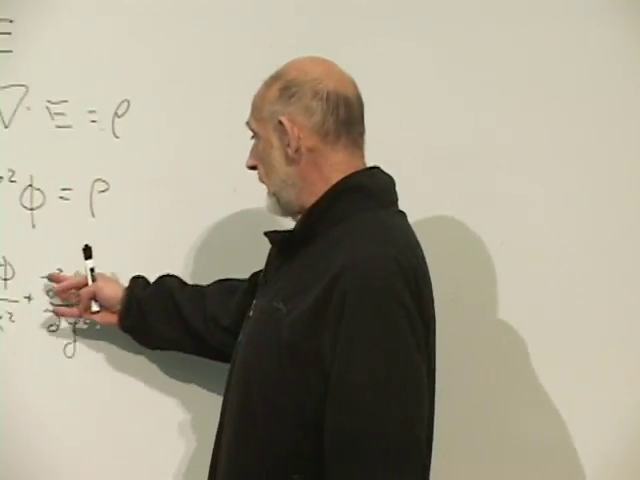
\includegraphics[width=0.70\textwidth]{lecture_08_figure_02.png}
  \caption{Das vollständige Paar der Cauchy--Riemann-Gleichungen einschließlich des relativen Minuszeichens.}
  \lectureframe{00:19:48}
  \label{fig:l08-cr-board}
\end{figure}

Die Vorlesung unterscheidet kurz verwandte Begriffe. Eine Funktion, die auf der gesamten endlichen komplexen Ebene holomorph ist, heißt ganz. Eine meromorphe Funktion kann isolierte Pole besitzen. Somit ist \(1/z\) außerhalb von \(z=0\) analytisch, aber nicht ganz.

\section{Harmonisch konjugierte Funktionen und konforme Geometrie}

Die Cauchy--Riemann-Gleichungen sind gekoppelte Differentialgleichungen erster Ordnung, implizieren aber getrennte Gleichungen zweiter Ordnung. Leiten wir \(\partial_xu=\partial_yv\) nach \(x\) ab, \(\partial_yu=-\partial_xv\) nach \(y\) und addieren wir die Ergebnisse:
\begin{align}
  \partial_x^2u&=\partial_x\partial_yv,\\
  \partial_y^2u&=-\partial_y\partial_xv,\\
  \therefore\qquad
  \partial_x^2u+\partial_y^2u&=0.
  \label{eq:l08-harmonic-u}
\end{align}
Vertauscht man in derselben Argumentation \(u\) und \(v\), so erhält man
\begin{equation}
  \partial_x^2v+\partial_y^2v=0.
  \label{eq:l08-harmonic-v}
\end{equation}
Real- und Imaginärteil einer analytischen Funktion sind daher harmonisch konjugiert. Zwei beliebige harmonische Funktionen ergeben nicht automatisch eine analytische Funktion; sie müssen weiterhin durch \eqref{eq:l08-cauchy-riemann} verknüpft sein.

\begin{figure}[H]
  \centering
  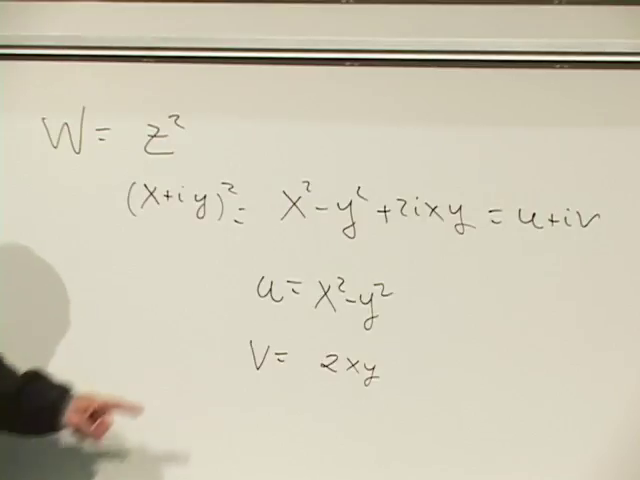
\includegraphics[width=0.68\textwidth]{lecture_08_figure_03.png}
  \caption{Die gemischten Ableitungen heben sich auf; übrig bleibt die Laplace-Gleichung für eine Komponente der analytischen Abbildung.}
  \lectureframe{00:23:09}
  \label{fig:l08-harmonic-board}
\end{figure}

Es gibt auch eine nützliche vektorielle Deutung. Für \(\mathbf F=(u,-v)\) besagen die beiden Cauchy--Riemann-Gleichungen, bis auf die gewählte Orientierungskonvention, dass sowohl die Divergenz als auch die zweidimensionale Rotation von \(\mathbf F\) verschwinden. Damit kehren wir wie angekündigt zur Elektrostatik zurück.

\subsection{Warum Winkel erhalten bleiben}

Schreiben wir zwei kleine komplexe Verschiebungen in Polarform:
\begin{equation}
  \delta z=\rho e^{i\theta},
  \qquad
  \Delta z=\rho'e^{i\theta'}.
\end{equation}
Ihr Quotient hat die Phase \(\theta-\theta'\), also genau den Winkel zwischen ihnen. Unter einer analytischen Abbildung gilt
\begin{equation}
  \frac{\delta w}{\delta z}
  =\frac{\Delta w}{\Delta z}
  =w'(z),
\end{equation}
da die Ableitung richtungsunabhängig ist. Umstellen ergibt
\begin{equation}
  \frac{\Delta z}{\delta z}
  =\frac{\Delta w}{\delta w}.
  \label{eq:l08-angle-ratio}
\end{equation}
Beide Seiten haben dieselbe Phase; daher ist der Winkel zwischen den ursprünglichen Intervallen gleich dem Winkel zwischen ihren Bildern.

\begin{figure}[H]
  \centering
  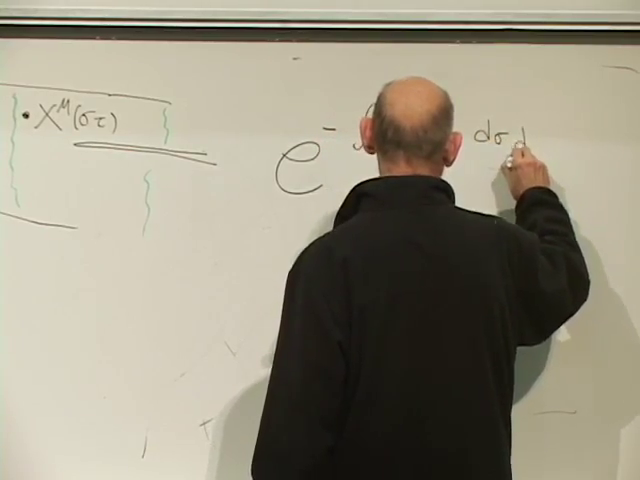
\includegraphics[width=0.70\textwidth]{lecture_08_figure_04.png}
  \medskip

  \begin{tikzpicture}[x=0.9cm,y=0.9cm,>=Latex]
    \begin{scope}
      \draw[->] (-0.2,0) -- (2.3,0);
      \draw[->] (0,-0.2) -- (0,2.1);
      \draw[very thick,blue!65!black,->] (0,0) -- (1.85,0.45)
        node[right] {\(\delta z\)};
      \draw[very thick,orange!75!black,->] (0,0) -- (0.72,1.65)
        node[above] {\(\Delta z\)};
      \draw (0.58,0.14) arc[start angle=14,end angle=66,radius=0.60];
      \node at (1.0,-0.55) {\(z\)-plane};
    \end{scope}
    \draw[->,thick] (3.0,0.9) -- (4.2,0.9)
      node[midway,above] {\(w(z)\)};
    \begin{scope}[xshift=5.0cm]
      \draw[->] (-0.2,0) -- (2.3,0);
      \draw[->] (0,-0.2) -- (0,2.1);
      \draw[very thick,blue!65!black,->] (0,0) -- (1.65,0.70)
        node[right] {\(\delta w\)};
      \draw[very thick,orange!75!black,->] (0,0) -- (0.48,1.62)
        node[above] {\(\Delta w\)};
      \draw (0.54,0.23) arc[start angle=23,end angle=74,radius=0.59];
      \node at (1.0,-0.55) {\(w\)-plane};
    \end{scope}
  \end{tikzpicture}
  \caption{Der Beweis an der Tafel und eine saubere lokale Rekonstruktion. Die Multiplikation
  mit \(w'(z)\) dreht und skaliert jede infinitesimale Richtung um denselben Betrag und erhält so ihren relativen Winkel.}
  \lectureframe{00:34:11}
  \label{fig:l08-angle-proof}
\end{figure}

Dieses lokale Argument setzt \(w'(z)\neq0\) voraus. An einem kritischen Punkt ist die Abbildung möglicherweise nicht lokal eineindeutig; dann muss man die Geometrie gesondert behandeln. Abseits solcher Punkte sind analytische und orientierungserhaltende konforme Abbildungen lokal dieselben Objekte.

\section{Beispiele zur Schulung des Blicks}

\subsection{Quadrieren und komplexe Konjugation}

Für \(w=z^2\) gilt
\begin{equation}
  (x+iy)^2=x^2-y^2+2ixy=u+iv,
\end{equation}
also
\begin{equation}
  u=x^2-y^2,
  \qquad
  v=2xy.
  \label{eq:l08-z-squared-components}
\end{equation}
Die zweiten Ableitungen von \(u\) sind \(2\) und \(-2\); diejenigen von \(v\) verschwinden jeweils. Beide Funktionen sind harmonisch, und direktes Ableiten bestätigt auch die Cauchy--Riemann-Gleichungen.

\begin{figure}[H]
  \centering
  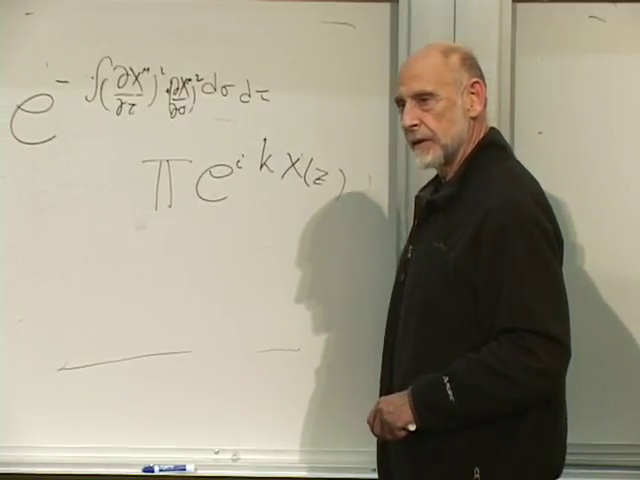
\includegraphics[width=0.72\textwidth]{lecture_08_figure_05.png}
  \caption{Die Quadrierungsabbildung, zerlegt in ihre reelle und imaginäre harmonische Komponente.}
  \lectureframe{00:36:45}
  \label{fig:l08-z-square-board}
\end{figure}

\begin{classroomqa}
\audiencequestion{Ist \(1/z\) ein Beispiel für eine nichtanalytische Funktion?
\lecturetimestamp{00:37:49}}
\lecturerresponse{Nur an einem einzigen Punkt. Die Funktion ist überall dort analytisch, wo \(z\neq0\) gilt, und hat am Ursprung einen Pol. Als Beispiel einer Abbildung, die die Cauchy--Riemann-Bedingung überall verletzt, eignet sich die komplexe Konjugation besser.}
\end{classroomqa}

Im Gegensatz dazu kehrt
\begin{equation}
  w=\bar z=x-iy
  \qquad\Longrightarrow\qquad
  u=x,\quad v=-y
\end{equation}
die Orientierung um. Ihre Ableitungen verletzen die erste Cauchy--Riemann-Gleichung aufgrund eines Vorzeichenfehlers; daher ist sie als Funktion von \(z\) nicht analytisch.

\begin{figure}[H]
  \centering
  \includegraphics[width=0.62\textwidth]{lecture_08_figure_06.png}
  \caption{Die komplexe Konjugation als bewusst gewähltes nichtanalytisches Gegenbeispiel.}
  \lectureframe{00:38:38}
  \label{fig:l08-conjugate-board}
\end{figure}

\subsection{Die Exponentialfunktion und ihre Umkehrfunktion}

\begin{classroomqa}
\audiencequestion{Wenn \(e^z\) analytisch ist, warum sollte dann auch ihre Umkehrfunktion \(\log z\) analytisch sein? \lecturetimestamp{00:40:38}}
\lecturerresponse{Wo die Umkehrfunktion existiert und \(w'(z)\neq0\) gilt, ist ihre Ableitung \(1/w'(z)\). Die Richtungsunabhängigkeit bleibt somit erhalten. Da der Logarithmus global mehrwertig ist, wählt man einen Zweig und schließt dessen Verzweigungspunkt und Schnitt aus. Die lokale konforme Aussage gilt weiterhin auf diesem gewählten Gebiet.}
\end{classroomqa}

Die Eulersche Formel liefert
\begin{equation}
  w=e^z=e^{x+iy}
  =e^x(\cos y+i\sin y),
\end{equation}
und damit
\begin{equation}
  u=e^x\cos y,
  \qquad
  v=e^x\sin y.
  \label{eq:l08-exponential-components}
\end{equation}
Zum Beispiel gilt \(\partial_xu=e^x\cos y=\partial_yv\), und die zweite Cauchy--Riemann-Gleichung folgt ebenso unmittelbar.

\begin{figure}[H]
  \centering
  \includegraphics[width=0.68\textwidth]{lecture_08_figure_07.png}
  \caption{Die reelle und imaginäre Komponente der Exponentialabbildung.}
  \lectureframe{00:42:23}
  \label{fig:l08-exponential-board}
\end{figure}

\section{Halbebene, Streifen, Zylinder und Kreisscheibe}

\subsection{Der Logarithmus macht aus dem Radius die Zeit}

Betrachten wir die rechte Halbebene, in der \(-\pi/2<\theta<\pi/2\) gilt, und schreiben wir
\begin{equation}
  z=re^{i\theta},
  \qquad
  w=\log z=\log r+i\theta.
  \label{eq:l08-log-map}
\end{equation}
Die Halbebene wird auf den unendlichen Streifen
\begin{equation}
  -\frac{\pi}{2}<\operatorname{Im}w<\frac{\pi}{2}.
\end{equation}
abgebildet. Strahlen mit festem \(\theta\) werden zu horizontalen Linien, während Halbkreise mit festem \(r\) zu vertikalen Linien werden. Der Ursprung wird auf \(\operatorname{Re}w=-\infty\) abgebildet und \(r=\infty\) auf \(\operatorname{Re}w=+\infty\).

\begin{figure}[H]
  \centering
  \includegraphics[width=0.75\textwidth]{lecture_08_figure_08.png}
  \caption{Der Logarithmus bildet die rechte Halbebene auf einen unendlichen Streifen ab: Polare Strahlen und Halbkreise ergeben ein orthogonales rechteckiges Gitter.}
  \lectureframe{00:47:48}
  \label{fig:l08-log-strip-board}
\end{figure}

Der Streifen ist die Standardweltfläche eines offenen Strings. Seine beschränkte Koordinate ist der Parameter entlang des Strings, die Verschiebung in der unbeschränkten Richtung ist die Weltflächenzeit. Unter der inversen Exponentialabbildung wird eine Zeitverschiebung zur Streckung \(z\mapsto e^a z\). Dieselbe Symmetrie erscheint also auf dem Streifen als Verschiebung und auf der Halbebene als gleichmäßige Expansion.

\begin{classroomqa}
\audiencequestion{Wohin wird ein bestimmter Wert wie \(r=1\) abgebildet, und sind die Koordinaten auf dem Streifen weiterhin polar? \lecturetimestamp{00:50:58}}
\lecturerresponse{Ein Kreis mit festem Radius wird zu einer vertikalen Linie bei \(\operatorname{Re}w=\log r\); insbesondere wird \(r=1\) auf die Mittellinie \(\operatorname{Re}w=0\) abgebildet. Polarkoordinaten beschreiben die \(z\)-Ebene. Auf der \(w\)-Ebene verwendet man gewöhnliche rechtwinklige Koordinaten \((\log r,\theta)\).}
\end{classroomqa}

Wird die gesamte punktierte Ebene durch \(\log z\) abgebildet, hat die Winkelkoordinate die Periode \(2\pi\). Daher werden die obere und untere Kante des resultierenden Streifens identifiziert: Es entsteht ein unendlicher Zylinder. Die Halbebene mit Rand beschreibt die Weltfläche eines offenen Strings; die gesamte Ebene ohne Rand und mit periodischem Winkel beschreibt einen Zylinder für einen geschlossenen String.

\begin{figure}[H]
  \centering
  \includegraphics[width=0.75\textwidth]{lecture_08_figure_09.png}
  \caption{Die Darstellung von Halbebene und Streifen sowie die periodische Identifizierung, durch die aus der gesamten punktierten Ebene ein Zylinder für einen geschlossenen String wird.}
  \lectureframe{00:54:23}
  \label{fig:l08-open-closed-board}
\end{figure}

\subsection{Eine Cayley-Abbildung auf die Einheitskreisscheibe}

Eine gebrochen-lineare, auch Möbius-Abbildung genannte Abbildung bildet die rechte Halbebene auf die Einheitskreisscheibe ab:
\begin{equation}
  w=\frac{z-1}{z+1}.
  \label{eq:l08-cayley}
\end{equation}
Sie bildet \(z=0\) auf \(-1\) ab, \(z=\infty\) auf \(+1\) und die imaginäre Achse auf \(|w|=1\). Für \(z=ir\) gilt
\begin{equation}
  \left|\frac{ir-1}{ir+1}\right|=1.
\end{equation}
Punkte mit \(\operatorname{Re}z>0\) liegen innerhalb des Kreises; die linke Halbebene wird nach außen abgebildet.
\editorialnote{Während der Herleitung an der Tafel wird die Kehrwertabbildung \((z+1)/(z-1)\) notiert, während die Abbildung auf das Innere der Kreisscheibe beschrieben wird. Diese Kehrwertabbildung hat denselben Einheitskreis als Rand, bildet die rechte Halbebene jedoch auf das Äußere ab. Gleichung \eqref{eq:l08-cayley} entspricht der Konvention für das Innere der Kreisscheibe und stimmt mit der angegebenen Geometrie überein.}

\begin{figure}[H]
  \centering
  \includegraphics[width=0.72\textwidth]{lecture_08_figure_10.png}
  \caption{Die gebrochen-lineare Konstruktion des Einheitskreisrandes. Die an der Tafel sichtbare Kehrwertkonvention vertauscht Inneres und Äußeres.}
  \lectureframe{00:58:38}
  \label{fig:l08-cayley-board}
\end{figure}

Möbius-Abbildungen bilden die verallgemeinerte Gesamtheit aus Kreisen und Geraden auf Kreise und Geraden ab. Das radiale und kreisförmige Gitter der Halbebene wird daher auf der Kreisscheibe zu zwei orthogonalen Scharen von Bögen. Ein gerader Durchmesser ist dabei der Grenzfall eines Kreises, dessen Mittelpunkt ins Unendliche gerückt ist.

\begin{classroomqa}
\audiencequestion{Sind die Bögen im Inneren der Kreisscheibe tatsächlich Kreise?
\lecturetimestamp{01:00:55}}
\lecturerresponse{Ja. Ihre Mittelpunkte liegen an verschiedenen Stellen, oft außerhalb der sichtbaren Kreisscheibe. Der Durchmesser ist der Grenzfall unendlichen Radius derselben Schar.}
\end{classroomqa}

\begin{classroomqa}
\audiencequestion{Bedeutet die Zeichnung der Kreisscheibe, dass es sich um eine Kugel handelt, und wohin kommt die andere Halbebene? \lecturetimestamp{01:01:21}}
\lecturerresponse{Die Zeichnung zeigt hier eine flache Kreisscheibe, keine Kugel. Die rechte Halbebene wird in ihr Inneres abgebildet, die linke Halbebene nach außen. Fügt man der gesamten komplexen Ebene den Punkt im Unendlichen hinzu, lässt sich diese erweiterte Ebene durch stereografische Projektion als Kugel darstellen; das ist eine andere globale Aussage.}
\end{classroomqa}

\begin{classroomqa}
\audiencequestion{Welche Kurven in der Kreisscheibe entsprechen den ursprünglichen radialen Strahlen und den Halbkreisen mit konstantem Radius? \lecturetimestamp{01:02:59}}
\lecturerresponse{Die positive reelle Achse wird zum Durchmesser zwischen \(-1\) und \(+1\). Andere Strahlen werden auf Kreisbögen abgebildet, die dieselben Randpunkte verbinden. Halbkreise mit festem Radius werden zur orthogonalen Schar, deren Bögen auf dem Einheitskreis beginnen und enden.}
\end{classroomqa}

\begin{figure}[H]
  \centering
  \includegraphics[width=0.72\textwidth]{lecture_08_figure_11.png}
  \caption{Geraden und Halbkreise der Halbebene werden in der Kreisscheibe zu orthogonalen Scharen aus Kreisen und Geraden.}
  \lectureframe{01:03:48}
  \label{fig:l08-circle-grid-board}
\end{figure}

\section{Die Weltfläche für vier Strings}

Kehren wir nun zur Streuung zurück. Zwei offene Strings treten ein, vereinigen sich zu einem String, propagieren über ein beliebiges Zeitintervall und spalten sich in zwei auslaufende Strings auf. In Streifenkoordinaten sieht die Weltfläche wie ein langes Band aus, das an beiden Enden geschlitzt ist---– das Bild des „Sportverbands“. Die Lebensdauer des Zwischenzustands wird nicht im Voraus festgelegt. Sie gehört zu den Verläufen, über die das Amplitudenintegral gebildet wird.

Seien \((\sigma,\tau)\) Koordinaten auf der Weltfläche und beschreibe
\begin{equation}
  X^\mu=X^\mu(\sigma,\tau)
  \label{eq:l08-embedding}
\end{equation}
ihre Lage in der Raumzeit. Die Indizes \(\sigma,\tau\) gehören zur zweidimensionalen Parameterfläche; der Index \(\mu\) bezeichnet Raumzeitkoordinaten. In der bosonischen Theorie gilt \(\mu=0,\ldots,25\); im Fall der Superstringtheorie gibt es zehn Raumzeitkoordinaten.

Nach einer Wick-Rotation haben die freien Einbettungsfelder die euklidische Wirkung
\begin{equation}
  S_E[X]
  =\frac{1}{4\pi\alpha'}\int_\Sigma d\sigma\,d\tau\,
  \left[
    \partial_\tau X^\mu\partial_\tau X_\mu
    +\partial_\sigma X^\mu\partial_\sigma X_\mu
  \right].
  \label{eq:l08-euclidean-action}
\end{equation}
Das zugehörige Pfadintegral summiert über alle Einbettungen der gewählten Weltfläche in die Raumzeit:
\begin{equation}
  \int\mathcal D X\,e^{-S_E[X]}.
  \label{eq:l08-bare-worldsheet-integral}
\end{equation}

\begin{figure}[H]
  \centering
  \includegraphics[width=0.74\textwidth]{lecture_08_figure_12.png}
  \caption{Die vervollständigte positive euklidische Weltflächenwirkung. Die beiden Ableitungsterme werden über alle Raumzeitkomponenten summiert.}
  \lectureframe{01:11:34}
  \label{fig:l08-action-board}
\end{figure}

Der geschlitzte Streifen hat einen zusammenhängenden Rand. Dank der konformen Freiheit lässt er sich daher als Kreisscheibe darstellen. Die vier entfernten Enden der Streifen werden zu vier markierten Punkten auf dem Rand. Eine Verschiebung der markierten Punkte verändert in Streifenkoordinaten den scheinbaren Abstand zwischen Vereinigung und Aufspaltung, nicht aber die zugrunde liegende Fläche oder Physik.

\begin{figure}[H]
  \centering
  \includegraphics[width=0.76\textwidth]{lecture_08_figure_13.png}
  \caption{Die Weltfläche in Form eines geschlitzten Streifens und ihre Darstellung als Kreisscheibe mit Randpunkten für die äußeren Strings.}
  \lectureframe{01:15:18}
  \label{fig:l08-bandage-disc-board}
\end{figure}

Die detaillierten Gitterlinien, mit denen diese konforme Abbildung veranschaulicht wird, haben keinen physikalischen Gehalt. Entscheidend sind die Topologie, der Rand und die markierten äußeren Punkte. Dieselbe Weltfläche lässt sich in verschiedene Kanalbilder strecken, ohne eine neue Wechselwirkung einzuführen.

\section{Äußere Zustände als Randeinsetzungen}

Das unverzierte Integral \eqref{eq:l08-bare-worldsheet-integral} gibt noch nicht an, welche Impulse ein- und austreten. Für einen skalaren Zustand eines offenen Strings mit Impuls \(k_i^\mu\) setzen wir auf dem Rand den Vertexoperator ein:
\begin{equation}
  V_i(z_i)=e^{\,i k_i\cdot X(z_i)},
  \qquad
  k_i\cdot X=k_{i\mu}X^\mu.
  \label{eq:l08-vertex}
\end{equation}
Der Punkt \(z_i\) gibt eine Position auf dem Rand der Weltfläche an. Er ist weder eine Raumzeitkoordinate noch eine Impulsrichtung.

\begin{figure}[H]
  \centering
  \includegraphics[width=0.72\textwidth]{lecture_08_figure_14.png}
  \caption{Das euklidische Gewicht im Inneren und das Produkt der Impulseinsetzungen am Rand sind als getrennte Faktoren dargestellt.}
  \lectureframe{01:18:58}
  \label{fig:l08-vertex-board}
\end{figure}

Für \(n\) äußere offene Strings lautet das schematische Streupostulat
\begin{equation}
  \begin{aligned}
    \mathcal A_n(k_1,\ldots,k_n)
    &=\int_{\mathcal M_{0,n}^{\partial}}\!d\mu(z_i)
      \int\mathcal D X\\
    &\quad\times e^{-S_E[X]}
      \prod_{i=1}^{n}e^{\,i k_i\cdot X(z_i)}.
  \end{aligned}
  \label{eq:l08-open-string-prescription}
\end{equation}
Das Funktionalintegral wird über Einbettungen \(X^\mu\) gebildet. Das endlichdimensionale Integral läuft über nicht äquivalente Positionen der Randeinsetzungen. Polarisationsfaktoren und das Eichfixierungsmaß sind in diesem Stadium weggelassen, wie auch in der Vorlesung.
\editorialnote{Eine vollständige eichfixierte Stringamplitude enthält außerdem den entsprechenden Geisterbeitrag, zustandsabhängige Vertexfaktoren, Kopplungskonstanten und eine Normierung. Gleichung
\eqref{eq:l08-open-string-prescription} hält die in dieser Vorlesung hergeleitete Abhängigkeit von Einbettungsfeldern und Positionen fest.}

\begin{classroomqa}
\audiencequestion{Wenn die äußeren Impulse festliegen, warum integriert man dann über sie? \lecturetimestamp{01:20:42}}
\lecturerresponse{Das tut man nicht. Die Größen \(k_i\) sind festgelegte Bezeichnungen der Streuamplitude. Integriert wird über die Einbettungsfelder und die Weltflächenpositionen \(z_i\), an denen diese festen Impulse eingesetzt werden. Das Integral über Letztere ersetzt das Integral über die Lebensdauer des Zwischenzustands im Streifenbild.}
\end{classroomqa}

\begin{classroomqa}
\audiencequestion{Liegt das Produkt der Vertexfaktoren im Pfadintegral, und ist es Teil der Wirkung? \lecturetimestamp{01:21:39}}
\lecturerresponse{Es multipliziert \(e^{-S_E}\) innerhalb des Funktionalintegrals. Man kann die Faktoren gleichwertig exponentieren und als lokalisierte Quellterme auffassen, die zur Wirkung hinzugefügt werden. Begrifflich handelt es sich jedoch um Vertexoperatoren und nicht um einen Bestandteil der freien Wirkung im Inneren.}
\end{classroomqa}

\begin{figure}[H]
  \centering
  \includegraphics[width=0.76\textwidth]{lecture_08_figure_15.png}
  \caption{Das Pfadintegral mit getrennten Faktoren \(e^{ik_i\cdot X(z_i)}\) für die einzelnen äußeren Teilchen.}
  \lectureframe{01:23:23}
  \label{fig:l08-full-prescription-board}
\end{figure}

\begin{classroomqa}
\audiencequestion{Warum enthält \(e^{ik\cdot X}\) nach der Wick-Rotation der Weltfläche weiterhin \(i\)? \lecturetimestamp{01:23:42}}
\lecturerresponse{Die Rotation verändert die Weltflächenzeit und wandelt das Gewicht im Inneren von \(e^{iS}\) in \(e^{-S_E}\) um. Das \(i\) in einer Impuls-Eigenfunktion ist die Fourier-Phase, die den Raumzeitimpuls kennzeichnet. Sie erfüllt eine andere Funktion und bleibt erhalten.}
\end{classroomqa}

\begin{classroomqa}
\audiencequestion{Bestimmt die Position \(z_i\) die Richtung des Impulsvektors? \lecturetimestamp{01:24:19}}
\lecturerresponse{Nein. Die Richtung ist in den Raumzeitkomponenten \(k_i^\mu\) codiert. Der Einsetzungspunkt \(z_i\) gibt an, an welcher Stelle dieser Impuls in die Weltflächenbeschreibung eingeht; \(X^\mu(z_i)\) gehört zu den Feldwerten, über die \(\mathcal D X\) gebildet wird.}
\end{classroomqa}

\begin{classroomqa}
\audiencequestion{Codieren die eingezeichneten Winkel der Verbandsschenkel die Richtungen der physikalischen Impulse? \lecturetimestamp{01:25:07}}
\lecturerresponse{Nein. Der Verband stellt den Parameterraum dar und nicht ein Bild des Strings in der physikalischen Raumzeit. Seine Schenkel können horizontal, geneigt oder konform gekrümmt gezeichnet werden. Die physikalischen Richtungen stecken in den Komponenten \(k^\mu\), während über \(X^\mu(\sigma,\tau)\) integriert wird.}
\end{classroomqa}

\section{Das gaußsche Integral als Elektrostatik}

Die Wirkung \eqref{eq:l08-euclidean-action} ist quadratisch in jeder Komponente \(X^\mu\), und sobald man die Exponentialfaktoren mit der Wirkung zusammenfasst, sind die Einsetzungen lineare Quellen. Das Funktionalintegral ist daher gaußsch. Am Sattelpunkt erfüllt jede Raumzeitkomponente eine Poisson-Gleichung der schematischen Form
\begin{equation}
  \nabla^2 X^\mu(z)
  \propto
  i\alpha'\sum_i k_i^\mu\,\delta(z-z_i),
  \label{eq:l08-electrostatic-source}
\end{equation}
mit der Randbedingung des offenen Strings am Rand der Kreisscheibe. Jedes \(X^\mu\) verhält sich wie ein unabhängiges elektrostatisches Potential, und jede Impulskomponente \(k_i^\mu\) wie die entsprechende Ladung am Ort \(z_i\).

\begin{figure}[H]
  \centering
  \includegraphics[width=0.76\textwidth]{lecture_08_figure_16.png}
  \caption{Die Kreisscheibe mit Randquellen lässt sich als ein unabhängiges zweidimensionales elektrostatisches Problem für jede Raumzeitkomponente deuten.}
  \lectureframe{01:28:58}
  \label{fig:l08-electrostatic-disc-board}
\end{figure}

Lösen wir das elektrostatische Problem, berechnen seine Energie, exponentieren die negative Energie und integrieren schließlich über die nicht äquivalenten Positionen der Ladungen. In der üblichen Normierung offener Strings liefert der Korrelator der Einbettungsfelder den Koba--Nielsen-Faktor
\begin{equation}
  \left\langle\prod_i e^{\,ik_i\cdot X(z_i)}\right\rangle
  \propto
  (2\pi)^D\delta^{(D)}\!\left(\sum_i k_i\right)
  \prod_{i<j}|z_i-z_j|^{2\alpha' k_i\cdot k_j}.
  \label{eq:l08-koba-nielsen}
\end{equation}
Die Delta-Funktion bringt die Impulserhaltung zum Ausdruck. Das Produkt enthält die elektrostatischen Paarenergien. Bei den vier hier verwendeten skalaren Randeinsetzungen wird das verbleibende Integral nach dem Fixieren dreier Positionen zum Euler'schen Beta-Integral, das in den vorangegangenen Vorlesungen auftrat.

\begin{classroomqa}
\audiencequestion{Gibt es sechsundzwanzig elektrostatische Energien oder nur eine?
\lecturetimestamp{01:30:53}}
\lecturerresponse{Für jede Raumzeitkomponente gibt es ein unabhängiges Potential und Feld. In einer orthonormalen Basis des Zielraums weisen ihre quadratischen Energien keine Kreuzterme auf. Die Beiträge werden zu einer Gesamtwirkung addiert, bevor man exponentiert.}
\end{classroomqa}

\begin{classroomqa}
\audiencequestion{Ist die Winkelkoordinate auf der Kreisscheibe der physikalische Streuwinkel? \lecturetimestamp{01:32:10}}
\lecturerresponse{Nein. Sie ist ein Positionsparameter auf der Weltfläche. Die nicht äquivalente Kombination steht mit dem Propagationsintervall des Zwischenzustands in Beziehung und wird integriert. Der physikalische Streuwinkel ist durch Lorentz-Invarianten ausgedrückt, die aus den festen Impulsen gebildet werden.}
\end{classroomqa}

\begin{classroomqa}
\audiencequestion{Warum versagt diese Konstruktion außerhalb der kritischen Dimension? \lecturetimestamp{01:32:35}}
\lecturerresponse{Die formalen gaußschen Integrale allein bilden nicht die gesamte Konsistenzbedingung. Bei der Eichfixierung entsteht eine konforme Anomalie, deren Materie- und Geisterbeiträge sich nur in der kritischen Dimension aufheben: \(D=26\) für den bosonischen String und \(D=10\) für den Superstring. Ohne diese Aufhebung geht die vermeintliche konforme Symmetrie der quantenmechanischen Weltfläche verloren.}
\end{classroomqa}

\begin{classroomqa}
\audiencequestion{Haben wir bereits drei große Raumdimensionen und kompakte zusätzliche Dimensionen vorausgesetzt? \lecturetimestamp{01:33:38}}
\lecturerresponse{Nein. Die Kompaktifizierung ist noch nicht Teil der Konstruktion. In diesem Stadium erstrecken sich die bosonischen Koordinaten weiterhin über alle sechsundzwanzig Richtungen des Zielraums, beziehungsweise über zehn im Fall der Superstringtheorie. Wie eine Teilmenge davon makroskopisch groß bleiben kann, ist Thema der nächsten Diskussion.}
\end{classroomqa}

\begin{classroomqa}
\audiencequestion{Besteht der Zusammenhang mit der Elektrostatik einfach darin, dass die Koordinaten die Laplace-Gleichung erfüllen? \lecturetimestamp{01:33:57}}
\lecturerresponse{Genau. Abseits der Einsetzungspunkte ist jedes \(X^\mu\) harmonisch; die Vertexoperatoren liefern Delta-Quellen. Das ist mathematisch dasselbe Randwertproblem wie das einer statischen zweidimensionalen Potentialverteilung mit Punktladungen, unabhängig davon, ob wir die Sprache der Elektrostatik verwenden.}
\end{classroomqa}

\subsection{Konforme Redundanz und die Anzahl der Moduli}

Die Kreisscheibe besitzt eine konforme Automorphismengruppe mit drei reellen Parametern, \(\mathrm{PSL}(2,\mathbb R)\). Daher lassen sich drei geordnete Randpunkte an bequemen Positionen fixieren. Bei vier äußeren Strings bleibt nur die vierte Position zu integrieren; bei \(n\) geordneten Randeinsetzungen verbleiben auf Baumebene
\begin{equation}
  n-3
  \label{eq:l08-n-minus-three}
\end{equation}
reelle Positionsintegrale.

\begin{classroomqa}
\audiencequestion{Gibt es vier unabhängige Winkelpositionen auf der Kreisscheibe? \lecturetimestamp{01:34:37}}
\lecturerresponse{Physikalisch gesehen nicht. Zunächst schreibt man vier Positionen hin, aber durch die konforme Symmetrie der Kreisscheibe lassen sich drei davon beliebig festlegen. Für die Amplitude mit zwei ein- und zwei auslaufenden Strings bleibt nur die relative Position der vierten übrig.}
\end{classroomqa}

\begin{figure}[H]
  \centering
  \includegraphics[width=0.72\textwidth]{lecture_08_figure_17.png}
  \caption{Vier Randeinsetzungen auf der Kreisscheibe. Die konforme Freiheit erlaubt es, drei davon zu fixieren; ein Modulus für vier Punkte bleibt übrig.}
  \lectureframe{01:35:18}
  \label{fig:l08-fix-three-board}
\end{figure}

\begin{classroomqa}
\audiencequestion{Was, wenn die beiden Aufspaltungspunkte in der Streifenzeichnung nicht auf derselben Höhe liegen? \lecturetimestamp{01:35:24}}
\lecturerresponse{Eine konforme Abbildung kann diese scheinbare Abweichung beseitigen. Verschiedene Zeichnungen sind Koordinatendarstellungen desselben Modulus. Die invariante Integration läuft über die verbleibende Randposition, gleichbedeutend mit dem Propagationsintervall.}
\end{classroomqa}

\begin{classroomqa}
\audiencequestion{Wie viele Positionsparameter bleiben bei mehr äußeren Teilchen übrig? \lecturetimestamp{01:36:00}}
\lecturerresponse{Fixiere drei Einsetzungspunkte mithilfe der konformen Symmetrie und integriere über die übrigen \(n-3\). Das ist die Anzahl der Randmoduli für eine geordnete offene Stringamplitude auf Baumebene.}
\end{classroomqa}

\begin{classroomqa}Wie hängt das mit der M-Theorie zusammen?
\audiencequestion{
\lecturetimestamp{01:36:37}}Noch gar nicht. Die hier behandelte Konstruktion beschreibt die perturbative Streuung offener Strings auf einer Weltfläche. Ihr Zusammenhang mit der M-Theorie erfordert spätere Dualitäten und nichtperturbative Ideen; die Frage wird daher ausdrücklich zurückgestellt.\lecturerresponse{
}
\end{classroomqa}

\begin{classroomqa}
\audiencequestion{Ergibt ein anderes vertikales oder gekreuztes Streifenbild eine andere Rechnung? \lecturetimestamp{01:36:49}}
\lecturerresponse{Nein. Man kann einen geeigneten Punkt festhalten und den verbleibenden Modul sein gesamtes Intervall durchlaufen lassen. Die Streifenbilder und das Integral über die Randpunkte auf der Kreisscheibe sind verschiedene Zerlegungen desselben Integrals. Deshalb lassen sich alle äußeren Strings symmetrisch behandeln.}
\end{classroomqa}

\section{Was das Rezept noch nicht löst}

Die Scheibenformel lässt sich unmittelbar auf mehr äußere Strings erweitern: Man fügt weitere Vertexoperatoren hinzu und integriert über ihre \(n-3\) nichtäquivalenten Randpositionen. Das ist ein präzises Rezept auf Baumebene für ein konsistentes Stringmodell, aber noch kein realistisches Modell der beobachteten Teilchenphysik. Der einfachen bosonischen Theorie fehlen die richtige Raumzeitdimension, und sie weist weitere physikalische Mängel auf. Superstrings verbessern das Spektrum und senken die kritische Dimension auf zehn; sechs räumliche Dimensionen müssen jedoch weiterhin kompaktifiziert werden.

\begin{classroomqa}
\audiencequestion{Stimmt dieses einfache Modell bereits mit Teilchenkollisionsexperimenten überein? \lecturetimestamp{01:39:06}}
\lecturerresponse{Nein. Die Resonanzstruktur ähnelt historisch der hadronischen Streuung, aber das sechsundzwanzigdimensionale bosonische Modell kann keine direkte Beschreibung der beobachteten Teilchen sein. Der Formalismus definiert Streuamplituden für das Modell; um mit der Natur übereinzustimmen, braucht es ein realistisches Spektrum, eine Kompaktifizierung, Wechselwirkungen und eine Wahl des Vakuums.}
\end{classroomqa}

\begin{classroomqa}
\audiencequestion{Werden durch Kompaktifizierung die zusätzlichen Dimensionen reduziert und realistische Teilchendaten erzeugt? \lecturetimestamp{01:41:10}}
\lecturerresponse{Sie kann die effektive makroskopische Dimension verringern und Teilchenspektren sowie Eichgruppen hervorbringen. Hier setzt auch ein großer Teil der mathematischen Schwierigkeiten ein. Viele konsistente Kompaktifizierungen sind bekannt, doch die Auswahl eines eindeutigen Modells der beobachteten Elementarteilchen ist weiterhin ungelöst.}
\end{classroomqa}

Die Vorlesung betont diesen Unterschied, statt eine abgeschlossene Theorie anzupreisen. Stringkonstruktionen sind mathematisch eindeutig und haben tiefgreifende Erkenntnisse über Gravitation und Geometrie geliefert; ihre Vielfalt ist jedoch selbst Teil des physikalischen Problems.

\begin{classroomqa}
\audiencequestion{Gibt es eine kurze Eselsbrücke dafür, warum die kritische Dimension der bosonischen Theorie sechsundzwanzig beträgt? \lecturetimestamp{01:43:19}}
\lecturerresponse{In der früheren Oszillatorrechnung wurde die regularisierte Nullpunktsumme \(1+2+3+\cdots=-1/12\) verwendet. Der Beitrag der transversalen Oszillatoren umfasst vierundzwanzig Richtungen; zählt man die beiden longitudinalen Raumzeitkoordinaten wieder hinzu, erhält man \(24+2=26\). Das ist eine Eselsbrücke zur früheren Konsistenzargumentation, keine neue Herleitung an dieser Stelle.}
\end{classroomqa}

\begin{classroomqa}
\audiencequestion{Sind die eingesetzten Impulse \(k_i\) selbst quantisiert?
\lecturetimestamp{01:43:46}}
\lecturerresponse{In einer nichtkompakten Raumzeit sind ihre Komponenten kontinuierlich. Quantisiert sind die Oszillatorstufe und damit das zulässige Massenspektrum im Quadrat. Kompakte Dimensionen können die entsprechenden Impuls- und Windungskomponenten quantisieren; das wird jedoch erst in der nächsten Erörterung behandelt.}
\end{classroomqa}
